\begin{center}
	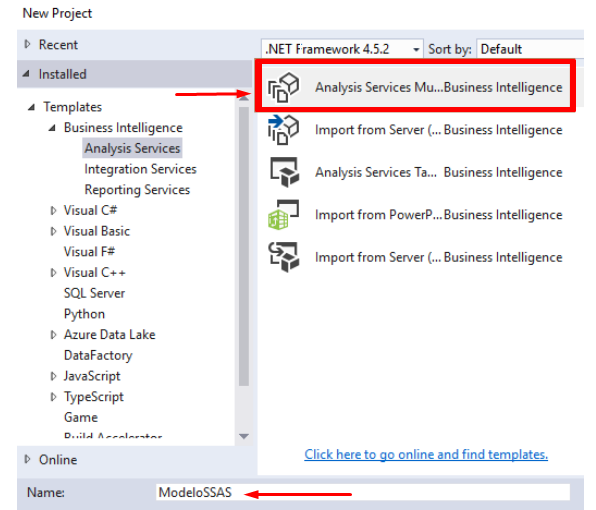
\includegraphics[width=8cm]{images/task1/img1}
\end{center}
\section{Creación de un Data Source}  
 En el Solution Explorer nos ubicamos en Data Sources y click derecho, seleccionando la opción de New
Data Source …
		

	\begin{center}
	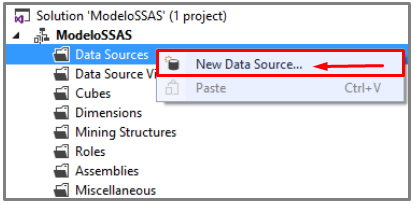
\includegraphics[width=8cm]{images/task1/img2}
	\end{center}	
Se nos abrirá una ventana de resumen. Click en Next:
	\begin{center}
	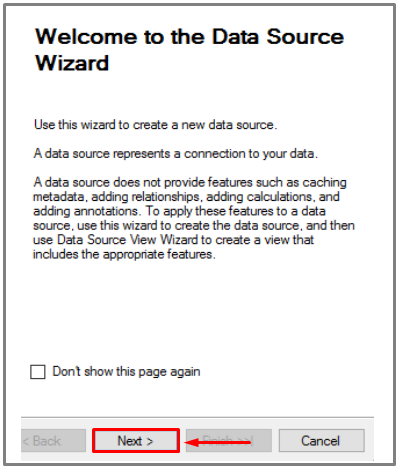
\includegraphics[width=8cm]{images/task1/img3}
	\end{center}	
Si es la primera vez que realizamos un proyecto de estos, no tendremos creadas conexiones. Click en New
para crear una nueva conexión hacia la base de datos Adventure Works DW:
	\begin{center}
	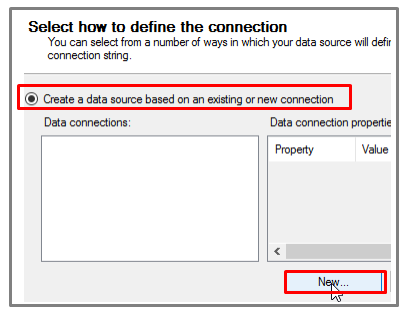
\includegraphics[width=8cm]{images/task1/img4}
    \end{center}	
Colocamos el nombre del Server donde se ubica la base de datos, en mi caso como es local coloco “.” ,
indicándole que es localhost. Ingresamos las credenciales y la base de datos Adventure Works DW 2014.
Luego Click en Ok:
	\begin{center}
	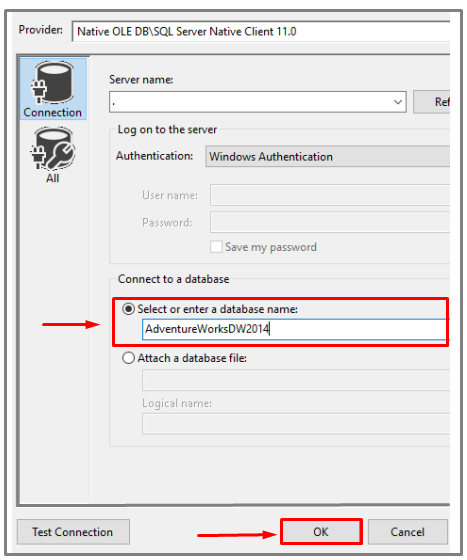
\includegraphics[width=8cm]{images/task1/img5}
    \end{center}	
Si todo está bien nos aparecerá la conexión creada en la sección de Data connections:
	\begin{center}
	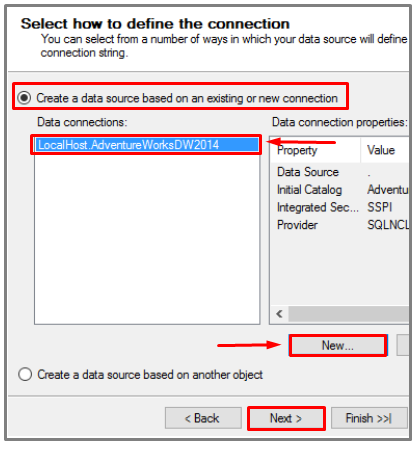
\includegraphics[width=8cm]{images/task1/img6}
    \end{center}	
En la ventana siguiente podemos definir las credenciales del Analysis Services y que utilizará para conectarse
al Data Source. En este caso utilizaremos las mismas credenciales del servicio. Para eso elegimos Use the
service account    
	\begin{center}
	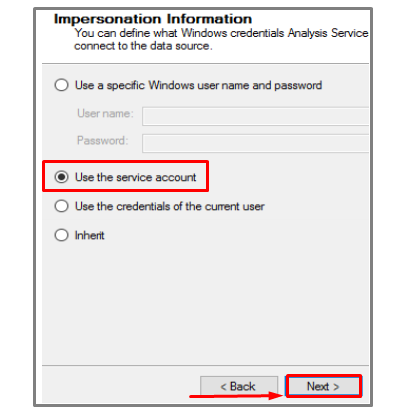
\includegraphics[width=8cm]{images/task1/img7}
    \end{center}	
Click en Next.
Colocamos un nombre para el Data Source y click en Finish:    
	\begin{center}
	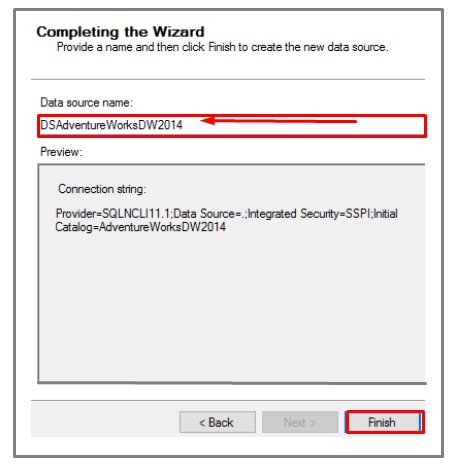
\includegraphics[width=8cm]{images/task1/img8}
    \end{center}	
   